\documentclass[dvipdfmx]{jsarticle}
\usepackage{amsmath, amssymb}
\usepackage{amsthm}
\usepackage{enumerate}
\usepackage[dvipdfmx]{graphicx}
\usepackage{tikz}
\usepackage{txfonts}
\usepackage{url}

\title{計算機数学 レポート (CA-1)}
\author{202020114 伊藤綾音}

\begin{document}
\maketitle

\noindent
課題1.\\
(補題3-41)\\
(1) フェルマーの小定理より $(a^{\frac{q}{p}})^{p} = a^{q} = a$ が成り立つため, これを $\frac{1}{p}$ 乗すれば得られる. \\
(2) 左辺を展開すると, $\displaystyle (a+b)^{p^{j}} = \sum_{i=0}^{p^{j}} \begin{pmatrix} p^{j} \\ i \end{pmatrix} a^{p^{j}-i}b^{i}$. 
右辺の初項と最終項以外の係数は $p$ の倍数であるため, $(a+b)^{p^{j}} = a^{p^{j}} + b^{p^{j}}$. \\
(定理3-42)\\
(十分性)\\
$f(x) = g(x)^{p}$ より $f^{\prime}(x) = p \cdot g(x)^{\prime} \cdot g(x)^{p-1} = 0$. \\
(必要性)\\
$f^{\prime}(x) = 0$ より, $f(x)$ の非ゼロの項の $x$ の指数は $p$ の倍数である. よって $^{\exists}k \in \mathbb{Z}_{>0}$ s.t. $\displaystyle f(x) = \sum_{i=0}^{k} a_{ip}x^{ip}$. 
ここで, $\displaystyle g(x) = \sum_{i=0}^{k} g_{i}x^{i}$, ただし $g_{i} = a_{ip}^{\frac{1}{p}} = a_{ip}^{p^{l-1}} \ (i = 0, \ldots, k)$ とすれば, 補題3-41より
\begin{eqnarray}
g(x)^{p} & = & \sum_{i=0}^{k} g_{i}^{p}x^{ip} \nonumber \\
         & = & \sum_{i=0}^{k} a_{ip}x^{ip} \nonumber \\
         & = & f(x). \nonumber
\end{eqnarray}

\noindent
課題2.\\ 
バールカンプのアルゴリズムを Risa/Asir \cite{asir}上で計算するプログラム report.rr を実装した. 
なお, report.rr は \url{https://github.com/yoreyore/0AJAD04-2020.git} にて公開している.
実行結果は下記の通りである. 

\begin{figure}[h]
\begin{center}
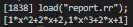
\includegraphics[scale=1]{./report.png}
\caption{report.rr の計算結果}
\end{center}
\end{figure}

\noindent
計算結果より, 求める既約因子は $x^{2}+2x+2, x^{3}+2x+1$ である.

\noindent
課題3.\\
オンデマンドで講義が受けられるのがありがたかったです. 
この講義に限らず, 今年度は未曽有の状況の中多くの場面で便宜を図っていただき, 大変お世話になりました。
まだまだ先の見えない状況が続きますが, 今後ともよろしくお願いいたします.

\begin{thebibliography}{9}
\bibitem{asir} M. Noro. 
A Computer Algebra System: Risa/Asir. 
In: M. Joswig M, N. Takayama (eds.), Algebra, Geometry and Software Systems, 147-162,  
Springer, 2003.
\end{thebibliography}

\end{document}